\scanpage{17}
$A\times_S U\simeq A_U$ can (\unsure{=vrai}). De plus, je dis qu'on a un isom $T_p(A)\simeq M$, qui recolle les $T_p(\unsure{A(s)})\simeq M(s)$. En effet, pour $\forall$ entier $n$, par le résultat déjà rappelé de pl. fid., on aura un isom \deleted{$T_p(A$} ${}_{p^n}A\simeq M(n)$ qui recolle les
\diagram{\begin{tikzcd}[ampersand replacement=\&,row sep=small,column sep=large]
{}_{p^n}(A_s)\arrow[r,phantom,"\unsure{\xrightarrow{\sim}|\simeq}"]\arrow[d,equal] \& \deleted{\unsure{{}_p}}M(s)(n)\arrow[d,equal]\\
({}_{p^n}A)_s \& (M(n))_s
\end{tikzcd}}
. Sur $U$, c'est l'isom. tautologique. On aura terminé.

Il reste à prouver la pleine fidélité précédente (on le laisse au lecteur), et le

\uline{Lemme}: Un ``syst local'' de schémas abéliens'' sur un schéma [\unsure{loc. n.th|loc. noeth}] \deleted{\unsure{a}} provient d'un schéma abélien.
\margin{\figure{\begin{tikzpicture}\node[draw,ellipse,align=center,inner sep=4pt] {Douteux,\\sans doute\\faux};\end{tikzpicture}}}
\margin{\figure{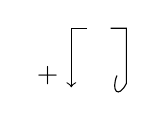
\begin{tikzpicture}[x=1cm,y=1cm]\node at (-.3,0){+};\draw[->](.2,.6)--(0,.6)--(0,-.15);\draw (.5,.6)--(.7,.6)--(.7,-.1) .. controls (.6,-.3) and (.5,-.2) .. (.58,0);\end{tikzpicture}} \unsure{inutile}?}

On peut supposer $S$ noethérien. \deleted{Soit} \inserted{On est ramené à prouver que} $U$ \deleted{\unsure{de} \unsure{plus}} pour un ouvert tel que l'on ait un schéma abélien $A_U$ sur $U$, et $t$ un pt maximal de $S-U=T$, on peut prolonger sur un voisinage $V$ de $t$.

Or \deleted{soit $B$} $V$ un voisinage ouvert de $t$, tel que $A(t)$ provient d'un schéma abélien sur $V$, \deleted{et \deleted{\unsure{soit}} tel que $V$ ne contient pas les $x\in\operatorname{Ass}O_S$ tels que $\unsure{\overline{\{x\}}|\bar x}\unsure{\not\ni|\not\supset}t$, \unsure{Je dis que pour} $\forall s\in V$, \unsure{il y a}}
\inserted{et tel que $B|U\cap V\simeq A_U$}
(isom compatible avec les isom $B\times\operatorname{Spec}O_{S,s}\simeq A(s)$ déjà connus, pour $s\in U\cap\operatorname{Spec}\underline O_{S,t}=:U(s)$). \deleted{Soit} On peut supposer que $x\in\operatorname{Ass}O_S$, $\bar x\unsure{\not\supset|\not\ni}\{t\}\Rightarrow x\notin V$, et que $V\cap\overline T\unsure{\subset|\in}\deleted{\unsure{\overline{\{t\}}}},\deleted{\unsure{t}}$. Soit alors $s\in V\cap\overline T$, donc \inserted{$s\in\overline{\{t\}}$}
\mspage{16}
